\chapter{行列式和线性方程组}

\section{二阶行列式和二元线性方程组}

\subsection{二阶行列式}
我们学过用消元法(代入消元或加减消元)解二元一次
方程组和三元一次方程组. 一次方程又叫\textbf{线性方程}, 一次方程
组又叫\textbf{线性方程组}. 本章学习线性方程组的行列式解法, 并对
解进行讨论。

一个二元线性方程组,当其中方程的个数与未知数的个
数相同时,它的一般形式可以写成
\[({\rm I})\begin{cases}
    a_1x+b_1y=c_1, & (1)\\
    a_2x+b_2y=c_2, & (2)
\end{cases}\]
其中$x,y$ 是未知数, $a_1,a_2,b_1,b_2$是未知数的系数, $c_1,c_2$是常
数项(在一般形式中, 我们把常数项写在方程的右边). 

若$x=x_1$, $y=y_1$适合方程组(I), 那么这一对有序实数
叫做方程组(I)的\textbf{一个解}, 记为
\[\begin{cases}
  x=x_1\\
y=y_1  
\end{cases}\]
或简记作$(x_1,y_1)$. 该方程组的所有的解构成的集合称为方程
组的\textbf{解集}. 

用加减消元法解这个方程组:
$(1)\x b_2-(2)\x b_1$,得
\begin{equation}
  (a_1b_2-a_2b_1)x=c_1b_2-c_2b_1\tag{3}
\end{equation}
$(2)\x a_1-(1)\x a_2$,得
\begin{equation}
  (a_1b_2-a_2b_1)y=a_1c_2-a_2c_1 \tag{4}
\end{equation}
应注意:方程组(3)(4)是方程组(I)的结果.因此,(I)的解一定适合(3)(4). 当$a_1b_2-a_2b_1\ne  0$时,方程组(3)(4)有唯一解.
\begin{equation}
\begin{cases}
  x=\frac{c_1b_2-c_2b_1}{a_1b_2-a_2b_1}\\
  y=\frac{a_1c_2-a_2c_1}{a_1b_2-a_2b_1}  
\end{cases}
\tag{5}
\end{equation}
可以验证:此时,(5)也适合方程组(I),所以当$a_1b_2-a_2b_1\ne  0$时,方程组(I)有唯一解(5).为了便于记忆(5),我们对它进行如下分析.

在公式(5)中,两个分母都是$a_1b_2-a_2b_1$,它只含有未知数的系数. 把未知数的系数按照它们在方程组中原来的位置排列成正方形(图8.1).
\begin{figure}[htp]
  \centering
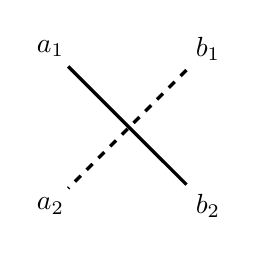
\begin{tikzpicture}
  \node(A) at (0,0){$a_1$};
  \node(B) at (2,0){$b_1$};
  \node(C) at (0,-2){$a_2$};
  \node(D) at (2,-2){$b_2$};
  \draw[very thick](A)--(D);
  \draw[dashed, very thick](B)--(C);
\end{tikzpicture}
  \caption{}
\end{figure}

可以看出:$a_1b_2-a_2b_1$恰是这样两项之和:第一项为正方形中实线表示的对角线(叫做\textbf{主对角线})上两数的乘积添上正号;
第二项为虚线表示的对角线(叫做\textbf{副对角线})上两数的乘积添上负号.由此,我们引进符号
\begin{equation}
  \begin{vmatrix}
    a_1&b_1\\
    a_2&b_2\\
  \end{vmatrix}\tag{6}
\end{equation}
并且规定它表示
\begin{equation}
  a_1b_2-a_2b_1\tag{7}
\end{equation} 
这时,符号(6)叫做\textbf{二阶行列式},(7)叫做(6)的\textbf{展开式}. $a_1,a_2,b_1,b_2$叫做行列式(6)的\textbf{元素}.这四个元素排成二行二列(横排叫行,竖排叫列).例如,$a_2$处在第二行第一列上;$b_1$处在第一行第二列上. 把(6)写成(7)叫做\textbf{按对角线法则}展开.

\begin{example}
  按对角线法则展开下列行列式,并化简:
\begin{multicols}{3}
\begin{enumerate}[(1)]
  \item $\begin{vmatrix}
    10&-9\\ -3&7
  \end{vmatrix}$
  \item $\begin{vmatrix}
    m+1& m+2\\ m & m+1
  \end{vmatrix}$
  \item $\begin{vmatrix}
    \sin x& \cos x\\ \cos x& -\sin x
  \end{vmatrix}$
\end{enumerate}
\end{multicols}
\end{example}

\begin{solution}
  \begin{enumerate}[(1)]
  \item $\begin{vmatrix}
    10&-9\\ -3&7
  \end{vmatrix}=10\x 7-(-3)(-9)=43$
  \item $\begin{vmatrix}
    m+1& m+2\\ m & m+1
  \end{vmatrix}=(m+1)^2-m(m+2)=1$
  \item $\begin{vmatrix}
    \sin x& \cos x\\ \cos x& -\sin x
  \end{vmatrix}=\sin^2 x-\cos^2 x=-1$
  \end{enumerate}
\end{solution}

\begin{thm}{问1}
  按对角线法则展开、化简下列行列式:
\begin{multicols}{2}
\begin{enumerate}[(1)]
  \item $\begin{vmatrix}
    5&6\\3&7
  \end{vmatrix}$
  \item $\begin{vmatrix}
   -3&-7\\-2&1
  \end{vmatrix}$
  \item $\begin{vmatrix}
    6a-b&2b\\ 3a&b
  \end{vmatrix}$
  \item $\begin{vmatrix}
    \log_a x & \log_a x\\m&n
  \end{vmatrix}$
\end{enumerate}
\end{multicols}
\end{thm}

\subsection{二元线性方程组的解的行列式表示法}
利用二阶行列式,同样可以把公式(5)中的两个分子也写
成行列式的形式,即
\[c_1b_2-c_2b_1=\begin{vmatrix}
  c_1&b_1\\c_2&b_2
\end{vmatrix},\qquad a_1c_2-a_2c_1=\begin{vmatrix}
  a_1&c_1\\ a_2&c_2
\end{vmatrix}\]
这样,当$a_1b_2-a_2b_1\ne 0$时,二元线性方程组(I)的解可以写成
\begin{equation}
  \begin{cases}
    x=\frac{\begin{vmatrix}
      c_1&b_1\\c_2&b_2
    \end{vmatrix}}{\begin{vmatrix}
      a_1&b_1\\a_2&b_2
    \end{vmatrix}}\\
    y=\frac{\begin{vmatrix}
      a_1&c_1\\a_2&c_2
    \end{vmatrix}}{\begin{vmatrix}
      a_1&b_1\\a_2&b_2
    \end{vmatrix}}
  \end{cases}\tag{8}
\end{equation}

为简便,通常用$D$、$D_x$、$D_y$分别表示(8)式中作为分母与分子的行列式\footnote{$D$是英语单词Determinant(行列式)的词头字母,通常用来表示行列式.}:
\[D=\begin{vmatrix}
  a_1&b_1\\a_2&b_2
\end{vmatrix},\qquad D_x=\begin{vmatrix}
  c_1&b_1\\c_2&b_2
\end{vmatrix},\qquad D_y=\begin{vmatrix}
  a_1&c_1\\a_2&c_2
\end{vmatrix}\]
行列式$D$是由方程组中未知数$x$、$y$的系数组成的,叫做这个方程组的\textbf{系数行列式}. $D$中第一列的元素$a_1$、$a_2$(即$x$的系数)分别用方程组的常数项$c_1$、$c_2$替换,就得到行列式$D_x$;$D$中第二列的元素$b_1$、$b_2$(即$y$的系数)分别用常数项$c_1$、$c_2$替换,就得到行列式$D_y$.

于是,当$D\ne 0$时,二元线性方程组(I)的唯一解可以写成
\begin{equation}
  \begin{cases}
    x=\frac{D_x}{D}\\[1ex]
   y=\frac{D_y}{D}
  \end{cases}\tag{9}
\end{equation}
或$\left(\frac{D_x}{D},\frac{D_y}{D}\right)$,方程组的解集就是$\left\{\left(\frac{D_x}{D},\frac{D_y}{D}\right)\right\}$.

由此可见,用行列式表示二元线性方程组的解的确简单好记.

\begin{example}
  利用行列式法解方程组
$\begin{cases}
  11x-2y+5=0,\\3x+7y+24=0.
\end{cases}  $
\end{example}

\begin{solution}
  解先把方程组写成一般形式
\[\begin{cases}
  11x-2y=-5 \\ 3x+7y=-24
\end{cases}\]
(这一步很必要,否则$c_1$、$c_2$的符号容易搞错)
由
\[\begin{split}
  D&=\begin{vmatrix}
    11&-2\\3&7
  \end{vmatrix}=77-3(-2)=83\ne 0\\
  D_x&=\begin{vmatrix}
    -5&-2\\-24&7
  \end{vmatrix}=-35-48=-83\\
  D_y&=\begin{vmatrix}
    11&-5\\3&-24
  \end{vmatrix}=-264-(-15)=-249\\
\end{split}\]
得
\[x=\frac{D_x}{D}=\frac{-83}{83}=-1,\qquad y=\frac{D_y}{D}=\frac{-249}{83}=-3\]
$\therefore\quad $方程组的解集是$\{(-1,-3)\}$.
\end{solution}

\begin{thm}{问2}
  用行列式法解方程组
\begin{multicols}{2}
\begin{enumerate}[(1)]
  \item $\begin{cases}
    7x-8y=10\\6x-7y=11
  \end{cases}$
  \item $\begin{cases}
    14x-6y+1=0\\
    3x+7y-6=0
  \end{cases}$
\end{enumerate}
\end{multicols}
\end{thm}

\subsection{二元线性方程组的解的讨论}
上面我们看到,当$D\ne 0$时,方程组(I)有唯一解(9),它仅仅是由方程组中未知数的系数和常数项表示的. 这就向我们暗示了一个问题:不经过解方程组,而仅仅根据方程组的系数和常数项能否确定方程组是否有解?在有解的情况下有多少解呢?(类似的问题我们在一元二次方程解的讨论中已经见过,所以在此提出这个问题并非偶然)

下面,我们分情况进行讨论\footnote{这里,我们是对形如$\begin{cases}
  a_1x+b_1y=c_1\\
  a_2x+b_2y=c_2
\end{cases}$的方程组进行讨论,对其中的系数不加任何限制。}. 为此,先把方程组(3)(4)写成
\[({\rm II})\begin{cases}
  D\cdot x=D_x & (10)\\
  D\cdot x=D_y &(11)
\end{cases}\]
由于方程组(I)的解都是方程组(II)的解,所以我们可以从(II)出发讨论方程组(I)的解的情况.
\begin{enumerate}
  \item 当$D\ne 0$时,由(II)可知,方程组(I)有唯一解;
\item 当$D=0$时,由(II)可知需考虑$D_x$、$D_y$:
\begin{enumerate}[(1)]
  \item 若$D_x$、$D_y$中至少有一个不为零.则(II)无解,也就是方程组(I)无解;
  \item 若$D_x=D_y=0$,例如$\begin{cases}
    2x+3y=4\\ 4x+6y=8
  \end{cases}$,我们再分两种情况讨论:
  \begin{enumerate}[(i)]
    \item $a_1$、$a_2$、$b_1$、$b_2$不全为零时,不失一般性,设$b_1\ne 0$,则由
\begin{equation}
  \begin{cases}
    D=a_1b_2-a_2b_1 =0\\
    D_x=c_1b_2-c_2b_1=0
  \end{cases}\Longrightarrow a_2=\frac{a_1b_2}{b_1},\quad c_2=\frac{c_1b_2}{b_1}  \tag{12}
\end{equation}    
把(12)代入(2),有
\[\frac{a_1b_2}{b_1}x+b_2y=\frac{c_1b_2}{b_1}\]
即
\begin{equation}
  \frac{b_2}{b_1}(a_1x+b_1y)=\frac{b_2}{b_1}c_1 \tag{13}
\end{equation}
这说明方程(1)的解必定适合方程(2). 因为方程(1)有无穷多解,所以方程组(I)有无穷多解.
\item $a_1$、$a_2$、$b_1$、$b_2$全为零时,这时若不全为零,方程组(I)无解;若$c_1$、$c_2$也全为零,则的任意一组值都同时适合方程(1)和(2),因此方程组(I)有无穷多解.
  \end{enumerate}
\end{enumerate}
\end{enumerate}

综合上述,结论是

\begin{thm}{定理}
  二元线性方程组$\begin{cases}
    a_1x+b_1y=c_1\\
    a_2x+b_2y=c_2
  \end{cases}$,也就是$\begin{cases}
    D\cdot x=D_x\\
    D\cdot y=D_y
  \end{cases}$
\begin{enumerate}
  \item 当$D\ne 0$时,有唯一解$\left(\frac{D_x}{D},\frac{D_y}{D}\right)$;
  \item 当$D=0$时:
\begin{enumerate}[(1)]
  \item 若$D_x$、$D_y$不全为零时,无解,
  \item 若$D_x$、$D_y$全为零时,
\begin{enumerate}[(i)]
  \item $a_1$、$a_2$、$b_1$、$b_2$不全为零,有无穷多解;
  \item $a_1$、$a_2$、$b_1$、$b_2$全为零,
\begin{itemize}
  \item 当$c_1,c_2$不全为零,无解;
  \item 当$c_1,c_2$全为零,无穷多解.
\end{itemize}
\end{enumerate}
\end{enumerate}
\end{enumerate}
\end{thm}

\begin{example}
  解关于$x,y$的线性方程组,并讨论:
\[\begin{cases}
  mx+y=m+1\\
  x+my=2m
\end{cases}\]
\end{example}

\begin{solution}
\[\begin{split}
D&=\begin{vmatrix}
  m&1\\1&m
\end{vmatrix}=m^2-1=(m+1)(m-1)\\
D_x&=\begin{vmatrix}
  m+1&1\\2m&m
\end{vmatrix}=m(m+1)-2m=(m-1)\\
D&=\begin{vmatrix}
  m&m+1\\1&2m
\end{vmatrix}=2m^2-(m+1)=(2m+1)(m-1)\\
\end{split}\]
\begin{enumerate}
  \item 当$D\ne 0$时,即$m\ne\pm 1$时,方程组有唯一解,其解集是$\left\{\left(\frac{m}{m+1},\frac{2m+1}{m+1}\right)\right\}$;
  \item 当$D=0$,即$m=\pm 1$时,
\begin{enumerate}[(1)]
  \item 当$m=-1$,这时$D=0$, $D_x=2\ne 0$,方程组无解,即解集为$\emptyset$;
  \item 当$m=1$时,$D_x=0$, $D_y=0$, $a_1\ne 0$,方程组有无穷多解. 这时方程组是
\[\begin{cases}
  x+y=2\\
  x+y=2  
\end{cases}\]
  若令$x=t$($t$为任意常数),则$y=2-t$,方程组的解集可以写成$\{(t,2-t)\}$($t$为任意常数).
\end{enumerate}
\end{enumerate}
\end{solution}

\section*{习题一}
\begin{center}
  \bfseries A
\end{center}

\begin{enumerate}
  \item 用对角线法则,展开行列式并化简:
\begin{multicols}{2}
\begin{enumerate}[(1)]
  \item $\begin{vmatrix}
    x-1& x^3\\ 1& x^2+x+1
  \end{vmatrix}$
  \item $\begin{vmatrix}
    \sin x-\sin y& \cos x+\cos y\\
    \cos x-\cos y& \sin x+\sin y
  \end{vmatrix}$
  \item $\begin{vmatrix}
    1-\sqrt{2} &2-\sqrt{3}\\
    2+\sqrt{3} & 1+\sqrt{2}
  \end{vmatrix}$
  \item $\begin{vmatrix}
    \log_a b& 1\\2&\log_b a
  \end{vmatrix}$
  \item $\begin{vmatrix}
    a-b&a^2-ab+b^2\\ a+b& a^2+ab+b^2
  \end{vmatrix}$
  \item $\begin{vmatrix}
    e^{x+y} &e^x-1\\
    e^x+1 & e^{x-y}
  \end{vmatrix}$
\end{enumerate}
\end{multicols}
  \item 利用行列式解下列方程组:
\begin{multicols}{2}
\begin{enumerate}[(1)]
  \item $\begin{cases}
    13x-7y-10=0\\
    19x+15y-2=0
  \end{cases}$
  \item $\begin{cases}
    \frac{7}{s}+\frac{9}{t}=3\\[1ex]
    \frac{17}{s}+\frac{7}{t}=5
  \end{cases}$
\end{enumerate}
\end{multicols}
  \item 利用行列式解下列关于$x,y$的方程组:
\begin{multicols}{2}
\begin{enumerate}[(1)]
  \item $\begin{cases}
    mx+y=2m+1\\x-my=2-m
  \end{cases}$
  \item $\begin{cases}
   x\cos A-y\sin A=\cos B\\
   x\sin A +y\cos A=\sin B
  \end{cases}$
\end{enumerate}
\end{multicols}
\end{enumerate}

\begin{center}
  \bfseries B
\end{center}

\begin{enumerate}\setcounter{enumi}{3}
  \item 不解方程组,判定下列方程组有唯一解、无解、还是有无穷多解:
\begin{multicols}{2}
\begin{enumerate}[(1)]
  \item $\begin{cases}
    2x+3y=7\\ 5x-2y=1
  \end{cases}$
  \item $\begin{cases}
    6x+9y=7\\ 4x+6y=2
  \end{cases}$
  \item $\begin{cases}
    4x-3y=5\\ 8x+6y=22
  \end{cases}$
  \item $\begin{cases}
    5x-15y=10\\ 3x-9y=6
  \end{cases}$
\end{enumerate}
\end{multicols}
  \item 判断$m$取什么值时,下列关于$x,y$的方程组有唯一解:
\begin{multicols}{2}
\begin{enumerate}[(1)]
  \item $\begin{cases}
    (m^2-1)x-(m+1)y=m+1\\
    m^2x-(m+1)y=m-1
  \end{cases}$
  \item $\begin{cases}
    x-(m^2-5)y=-1\\
    (m+1)x- (m+1)^2 y=1
  \end{cases}$
\end{enumerate}
\end{multicols}
\item 解下列关于$x,y$的方程组,并进行讨论:
\begin{multicols}{2}
\begin{enumerate}[(1)]
  \item $\begin{cases}
    x+(m-1)y=1\\ (m-1)x+y=2
  \end{cases}$
  \item $\begin{cases}
    4x+my=m\\ mx+y=1
  \end{cases}$
\end{enumerate}
\end{multicols}
\end{enumerate}

\section{关于三元线性方程组的猜想}
二阶行列式的引入使二元线性方程组的求解和讨论大为简化.成功的喜悦和好奇心驱使我们进一步考虑能否用类似的办法去简化三元线性方程组的求解和讨论呢?具体讲,是否可以引入“三行三列”的行列式,由三元线性方程组
\begin{equation}
  \begin{cases}
    a_1x+b_1y+c_1z=d_1\\
    a_2x+b_2y+c_2z=d_2\\
    a_3x+b_3y+c_3z=d_3\\
  \end{cases}\mathop{\Longrightarrow}^{\text{推出}}\begin{cases}
    D\cdot x =D_x\\
    D\cdot y =D_y\\
    D\cdot z =D_z\\
  \end{cases}\tag{*}
\end{equation}
其中
\[D=\begin{vmatrix}
  a_1&b_1&c_1\\
  a_2&b_2&c_2\\
  a_3&b_3&c_3\\
\end{vmatrix},\quad D_x=\begin{vmatrix}
  d_1&b_1&c_1\\
  d_2&b_2&c_2\\
  d_3&b_3&c_3\\
\end{vmatrix}\]
\[D_y=\begin{vmatrix}
  a_1&d_1&c_1\\
  a_2&d_2&c_2\\
  a_3&d_3&c_3\\
\end{vmatrix},\quad D_z=\begin{vmatrix}
  a_1&b_1&d_1\\
  a_2&b_2&d_2\\
  a_3&b_3&d_3\\
\end{vmatrix}\]
当然必须恰当地规定$D$的展开式是什么.如果这一“猜想”得以实现,三元线性方程组的问题就基本解决了,就有可能进一步去考虑四元、五元以至$n$元线性方程组的问题了.

\begin{thm}
  {问1} 你能够把这一猜想付诸实现吗?这里关键是规定$D$的展开式(类比“二元”的线索去发现)和实现(*)式的改写.
\end{thm}

\section{三阶行列式及其性质}
引进符号
\begin{equation}
  \begin{vmatrix}
    a_1&b_1&c_1\\
    a_2&b_2&c_2\\
    a_3&b_3&c_3\\
  \end{vmatrix}\tag{1}
\end{equation}
并规定它表示
\begin{equation}
  a_1b_2c_3+a_2b_3c_1+a_3b_1c_2-a_3b_2c_1-a_2b_1c_3-a_1b_3c_2 \tag{2}
\end{equation}

(1)称为\textbf{三阶行列式}.它有三行三列,共有9个元素.(2)称为(1)的\textbf{展开式},共有六项.

三阶行列式按对角线法则展开,如图8.2.
\begin{figure}[htp]
  \centering
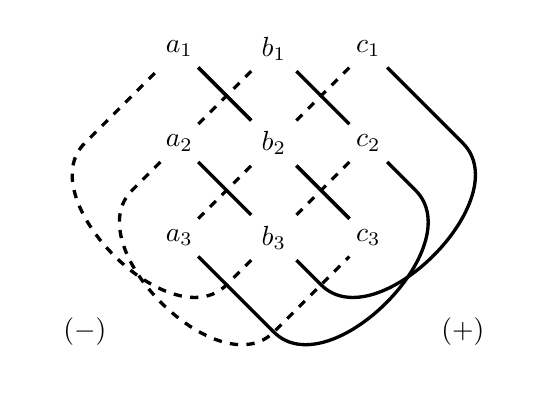
\begin{tikzpicture}[very thick, scale=1.2]
\node (A1) at (-1,1){$a_1$};
\node (B1) at (0,1){$b_1$};
\node (C1) at (1,1){$c_1$};
\node (A2) at (-1,0){$a_2$};
\node (B2) at (0,0){$b_2$};
\node (C2) at (1,0){$c_2$};
\node (A3) at (-1,-1){$a_3$};
\node (B3) at (0,-1){$b_3$};
\node (C3) at (1,-1){$c_3$};
\draw (A1)--(B2)--(C3);
\draw (A2)--(B3)--(1-.5,-2+.5)[bend left=-90]to (2,0)-- (C1);
\draw (B1)--(C2)--(1+.5,0-.5)[bend left=90]to (0,-2)--(A3);
\draw (A1)--(B2)--(C3);

\draw [dashed](A3)--(B2)--(C1);
\draw [dashed](C2)--(B3)--(-.5,-1.5)[bend left=90]to (-2,0)-- (A1);
\draw[dashed] (B1)--(A2)--(-1-.5,0-.5)[bend left=-90]to (0,-2)--(C3);

\node at (-2,-2){$(-)$};
\node at (2,-2){$(+)$};

\end{tikzpicture}
  \caption{}
\end{figure}


图中实线上三个元素的积,添上正号;虚线上三个元素的积,添上负号. 容易看出,三阶行列式的值就是这六项的和.

\begin{example}
  用对角线法则计算行列式$\begin{vmatrix}
    3&-2&1\\ -2&1&3\\2&0&-2
  \end{vmatrix}$
\end{example}

\begin{solution}
\[\begin{split}
  \begin{vmatrix}
    3&-2&1\\ -2&1&3\\2&0&-2
  \end{vmatrix}&=3\x1\x(-2)+(-2)\x0\x1+2\x(-2)\x3\\
  &\qquad 
  -2\x1\x1-(-2)\x(-2)\x(-2)-3\x0\x3\\
 & =-6+0-12-2+8-0\\
  &=-12
\end{split}\]
\end{solution}

\section*{习题二}
\begin{center}
  \bfseries A
\end{center}
\begin{enumerate}
  \item 用对角线法则计算:
\begin{multicols}{2}
\begin{enumerate}[(1)]
  \item $\begin{vmatrix}
    1&5&7\\2&0&-4\\-3&1&6
  \end{vmatrix}$
  \item $\begin{vmatrix}
    2&-3&1\\4&-1&7 \\-1&5&2
  \end{vmatrix}$
\end{enumerate}
\end{multicols}
  \item 用对角线法则展开下列行列式,并化简:
\begin{multicols}{2}
\begin{enumerate}[(1)]
  \item $\begin{vmatrix}
    0&a&b\\a&0&c\\b&c&0
  \end{vmatrix}$
  \item $\begin{vmatrix}
    x&y&z\\ z&x&y\\y&z&x
  \end{vmatrix}$
  \item $\begin{vmatrix}
    a&b&c\\2a&2b&2c\\m&n&l
  \end{vmatrix}$
  \item $\begin{vmatrix}
    1&-a&-b\\a&1&-c\\b&c&1
  \end{vmatrix}$
\end{enumerate}
\end{multicols}
\end{enumerate}

三阶行列式按对角线法则展开计算是较繁的.为了简化计算和理论研究的需要,我们以三阶行列式为例学习行列式
的性质.

\begin{thm}
  {性质1} 把各行变为相应的列(就是把第$i$行变为第$i$列,$i=1,\ldots,2,3$)所得行列式与原行列式等值(简述成:行列互换值不变). 即
\[\begin{vmatrix}
  a_1&b_1&c_1\\
  a_2&b_2&c_2\\
  a_3&b_3&c_3\\
\end{vmatrix}=\begin{vmatrix}
  a_1&a_2&a_3\\
  b_1&b_2&b_3\\
  c_1&c_2&c_3\\
\end{vmatrix}\]
\end{thm}

\begin{proof}
  按对角线法则分别把它们展开,比较相应项,即可得证.
\end{proof}

性质1的价值在于:对行成立的定理,对列也一定成立,反之亦然(这叫做行与列的对偶性). 因此,下面各条性质我们只对“行”叙证,对“列”的情况,由性质1保证,也就不述自明了.

\begin{thm}
 {性质2} 把任意两行对调,所得行列式与原行列式绝对值相等,符号相反(简述成:两行互换值相反). 
\end{thm}

\begin{proof}
  先证二、三两行互换值相反. 即
\[\begin{vmatrix}
  a_1&b_1&c_1\\
  a_2&b_2&c_2\\
  a_3&b_3&c_3\\
\end{vmatrix}=-\begin{vmatrix}
  a_1&b_1&c_1\\
  a_3&b_3&c_3\\
  a_2&b_2&c_2\\
\end{vmatrix}\]
按对角线法则展开比较两边即可获证.
\end{proof}

其他情况同理可证.

\begin{thm}
  {推论1} 若有两行对应元素相同,行列式的值等于零(简述成:两行相同值为零).
\end{thm}

\begin{proof}
  设$D$有两行对应元素相同,把这两行对调,所得仍是原行列式$D$,但据性质2,应有
$$D=-D\Longrightarrow D=0$$
\end{proof}

\begin{thm}
 {性质3} 某行元素都乘常数$k$,等于原行列式乘$k$(简述成:某行乘$k$,值$k$倍). 
\end{thm}

\begin{proof}
  先证第二行乘$k$等于原行列式乘$k$,即
\[\begin{vmatrix}
  a_1&b_1&c_1\\
  ka_2&kb_2&kc_2\\
  a_3&b_3&c_3\\
\end{vmatrix}=k\begin{vmatrix}
  a_1&b_1&c_1\\
  a_2&b_2&c_2\\
  a_3&b_3&c_3\\
\end{vmatrix}\]
两边都按对角线法则展开比较即明.
\end{proof}

\begin{thm}
{推论2} 某行有公因子,可以提到行列式外.
\end{thm}

\begin{example}
  计算$\begin{vmatrix}
    \frac{1}{2}&\frac{1}{2}&-1\\[1ex]
    \frac{1}{3}&\frac{2}{3}&-\frac{2}{3}\\[1ex]
    \frac{2}{5}&\frac{3}{5}&-\frac{1}{5}
  \end{vmatrix}$
\end{example}

\begin{solution}
\[\begin{split}
  \text{原行列式}&=(-1)\x \frac{1}{2}\x\frac{1}{3}\x\frac{1}{5}\x \begin{vmatrix}
    1 &1&2\\1&2&2\\2&3&1
  \end{vmatrix}\qquad \text{(推论2)}\\
  &=-\frac{1}{30}(2+6+4-8-1-6)=-\frac{1}{30}\times (-3)\\
  &=\frac{1}{10}
\end{split}\]
\end{solution}

\begin{rmk}
  由此可见,运用推论2提公因式,可简化计算.
\end{rmk}

\begin{thm}
{推论3} 若某行所有元素全为零,那么行列式的值为零(简述成:某行为零,值为零).  
\end{thm}

\begin{thm}
  {性质4} 若有两行对应元素成比例,那么行列式的值为
零(简述成两行成比例,值为零).
\end{thm}

\begin{proof}
  先证第一、二行成比例,行列式值为零.此时有
$$D=\begin{vmatrix}a_1&b_1&c_1\\ka_1&kb_1&kc_1\\a_3&b_3&c_3\end{vmatrix},$$
据推论 2 与推论 1 有
$$D=k\begin{vmatrix}a_1&b_1&c_1\\a_1&b_1&c_1\\a_3&b_3&c_3\end{vmatrix}=k\cdot0=0.$$
其他情况,同理可证。
\end{proof}

\begin{thm}
  {性质5} 若某行元素都是二项式,那么原行列式等于把这些二项式各取一项作成相应行,而其余行不变的两个行列式的和(简述成:某行都是二项式,可相应分成两个行列式之和).
\end{thm}

\begin{proof}
  我们先证明
\begin{equation}
  \begin{vmatrix}a_1+a_1'&b_1+b_1'&c_1+c_1'\\a_2&b_2&c_2\\a_3&b_3&c_3\end{vmatrix}=\begin{vmatrix}a_1&b_1&c_1\\a_2&b_2&c_2\\a_3&b_3&c_3\end{vmatrix}+\begin{vmatrix}{a_1}'&{b_1}'&{c_1}'\\{a_2}&{b_2}&{c_2}\\{a_3}&{b_3}&{c_3}\end{vmatrix}\tag{*}
\end{equation}
\[\begin{split}
  \text{左边}&=(a_{1}+a_{1}^{\prime})b_{2}c_{3}+a_{2}b_{3}(c_{1}+c_{1}^{\prime})+a_{3}(b_{1}+b_{1}^{\prime})c_{2}\\
&\qquad -a_{3}b_{2}(c_{1}+c_{1}^{\prime})-a_{2}(b_{1}+b_{1}^{\prime})c_{3}-(a_{1}+a_{1}^{\prime})b_{3}c_{2}\\
&=(a_{1}b_{2}c_{3}+a_{2}b_{3}c_{1}+a_{3}b_{1}c_{2}-a_{3}b_{2}c_{1}-a_{2}b_{1}c_{3}-a_{1}b_{3}c_{2})\\
&\qquad +(a_{1}^{\prime}b_{2}c_{3}+a_{2}b_{3}c_{1}^{\prime}+a_{3}b_{1}^{\prime}c_{2}-a_{3}b_{2}c_{1}^{\prime}-a_{2}b_{1}^{\prime}c_{3}-a_{1}^{\prime}b_{3}c_{2})\\
&=\begin{vmatrix}a_1&b_1&c_1\\a_2&b_2&c_2\\a_3&b_3&c_3\end{vmatrix}+\begin{vmatrix}{a_1}'&{b_1}'&{c_1}'\\{a_2}&{b_2}&{c_2}\\{a_3}&{b_3}&{c_3}\end{vmatrix}.
\end{split}\]

$\therefore\quad $(*)成立. 其余情况同理可证.
\end{proof}

\begin{example}
  求证
$D=\begin{vmatrix}1&x^{2}&a^{2}+x^{2}\\1&y^{2}&a^{2}+y^{2}\\1&z^{2}&a^{2}+z^{2}\end{vmatrix}=0.$
\end{example}

\begin{proof}
  $$D=\begin{vmatrix}1&x^2&a^2\\1&y^2&a^2\\1&z^2&a^2\end{vmatrix}+\begin{vmatrix}1&x^2&x^2\\1&y^2&y^2\\1&z^2&z^2\end{vmatrix}=0.$$
(据性质4, 第一个行列式为零, 据推论1, 第二个行列式也为零)
\end{proof}


由此可见,运用行列式性质确能简化计算.

\begin{thm}
{性质6} 某行各元素同乘以$k$, 加到另--行的对应元素上,所得行列式与原行列式等值(简述成:某行乘$k$加到另一行,值不变).  
\end{thm}

\begin{proof}
  先证明把第二行各元素同乘$k$, 加到第一行对应
元素上,行列式值不变,即
$$\begin{vmatrix}a_1+ka_2&b_1+kb_2&c_1+kc_2\\a_2&b_2&c_2\\a_3&b_3&\cdot&c_3\end{vmatrix}=\begin{vmatrix}a_1&b_1&c_1\\a_2&b_2&c_2\\a_3&b_3&c_3\end{vmatrix}.$$
\[\begin{split}
  \text{左边}&=\begin{vmatrix} a_1& b_1& c_1\\ a_2& b_2& c_2\\ a_3& b_3& c_3\end{vmatrix} + \begin{vmatrix} ka_2& kb_2& kc_2\\ a_2& b_2& c_2\\ a_3& b_3& c_3\end{vmatrix}\qquad  \text{(性质5)}\\
  &= \begin{vmatrix} a_1& b_1& c_1\\ a_2& b_2& c_2\\ a_3& b_3& c_3\end{vmatrix} \qquad  \text{(性质 4)}
\end{split}\]
其余情况同理可证.
\end{proof}

\begin{example}
  利用行列式性质,计算:
\begin{multicols}{2}
\begin{enumerate}[(1)]
  \item $\begin{vmatrix}3&2&6\\8&10&9\\6&-2&21\end{vmatrix}$
  \item $\begin{vmatrix} 10& - 2& 7\\ - 15& 3& 2\\ - 5& 4& 9\end{vmatrix} $
\end{enumerate}
\end{multicols}
\end{example}

\begin{solution}
\[\begin{split}
(1)\quad \begin{vmatrix}3&2&6\\8&10&9\\6&-2&21\end{vmatrix}&=3\times2\times\begin{vmatrix}3&1&2\\8&5&3\\6&-1&7\end{vmatrix}\qquad\text{(推论 2)}\\
&=6\times \begin{vmatrix} 3& 1+ 2& 2\\ 8& 5+ 3& 3\\ 6& - 1+ 7& 7\end{vmatrix} \qquad \text{(性质 6)} \\
&= 6\times \begin{vmatrix} 3& 3& 2\\ 8& 8& 3\\ 6& 6& 7\end{vmatrix} = 0 \qquad \text{(推论 1)}
\end{split}\]
\[\begin{split}
  (2)\quad \begin{vmatrix} 10& - 2& 7\\ - 15& 3& 2\\ - 5& 4& 9\end{vmatrix} &=5\times \begin{vmatrix} 2& - 2& 7\\ - 3& 3& 2\\ - 1& 4& 9\end{vmatrix} \qquad \text{(推论 2)}\\
  &=5\times \begin{vmatrix} 2& - 2+2& 7\\ - 3& 3+(-3)& 2\\ - 1& 4+(-1)& 9\end{vmatrix} \qquad \text{(性质6)}\\
  &=5\times \begin{vmatrix} 2& 0& 7\\ - 3& 0& 2\\ - 1& 3& 9\end{vmatrix} =5\times (-63-12)=-375.
\end{split}\]
\end{solution}

\begin{note}
在计算行列式时,为了简化计算,首先应注意使行列式值为零的几个定理或推论(推论 1、推论 3、性质 4)的条件是否满足,或者能否化到这三种情况——此时立刻可断定行列式值为零;其次,看看是否可提公因式,或用性质 6 把某行(或某列)的两个元素一起都变为零,从而简化计算;第三, 使行列式做等值变形的几个定理应熟练掌握.
\end{note}

\begin{example}
  利用行列式性质,证明
\begin{multicols}{2}
\begin{enumerate}[(1)]
  \item $\begin{vmatrix}0&a&b\\-a&0&c\\-b&-c&0\end{vmatrix}=0;$
  \item $\begin{vmatrix}a+b&c&-a\\a+c&b&-c\\b+c&a&-b\end{vmatrix}=\begin{vmatrix}b&a&c\\a&c&b\\c&b&a\end{vmatrix}.$
\end{enumerate}  
\end{multicols}
\end{example}

\begin{proof}
\[\begin{split}
  (1)\quad \begin{vmatrix} 0& a& b\\ - a& 0& c\\ - b& - c& 0\end{vmatrix} &= \begin{vmatrix} 0& - a& - b\\ a& 0& - c\\ b& c& 0\end{vmatrix}\qquad \text{(性质 1)}\\
  &=-\begin{vmatrix}0&a&b\\-a&0&c\\-b&-c&0\end{vmatrix}\qquad \text{(推论2)}
\end{split} \]
$\therefore\quad \begin{vmatrix} 0& a& b\\ - a& 0& c\\ - b& - c& 0\end{vmatrix}=0.$

\[\begin{split}
  (2)\quad \begin{vmatrix}a+b&c&-a\\a+c&b&-c\\b+c&a&-b\end{vmatrix}&=\begin{vmatrix}b&c&-a\\a&b&-c\\c&a&-b\end{vmatrix}\qquad \text{(性质 6)}\\
  &=- \begin{vmatrix} b& c& a\\ a& b& c\\ c& a& b\end{vmatrix}\qquad \text{(推论 2)} \\
  &= \begin{vmatrix} b& a& c\\ a& c& b\\ c& b& a\end{vmatrix}\qquad \text{(性质 2)}
\end{split}\]
\end{proof}

\section*{习题三}
\begin{center}
  \bfseries A
\end{center}
\begin{enumerate}
  \item 利用行列式的性质计算:
\begin{multicols}{3}
\begin{enumerate}[(1)]
  \item $\begin{vmatrix}3&2&6\\8&10&9\\6&-2&21\end{vmatrix}$
  \item $\begin{vmatrix}10&-2&7\\-15&3&2\\-5&4&9\end{vmatrix}$
  \item $\begin{vmatrix}1&3&4\\10&1&11\\7&1&8\end{vmatrix}$
  \item $\begin{vmatrix}3&49&4\\2&28&4\\4&35&8\end{vmatrix}$
  \item $\begin{vmatrix}
    \frac{2}{3}&\frac{2}{3}&3\\7&5&14\\
    \frac{1}{3}&\frac{1}{5}&\frac{4}{15}
  \end{vmatrix}$
  \item $\begin{vmatrix}
    1&4&7\\2&5&8\\3&6&9
  \end{vmatrix}$
\end{enumerate}
\end{multicols}

\item 利用行列式的性质计算:
\begin{multicols}{2}
\begin{enumerate}[(1)]
  \item $\begin{vmatrix}a&a&a\\-a&a&x\\-a&-a&x\end{vmatrix}$
  \item $\begin{vmatrix}1&a&b+c\\1&c&c+a\\1&c&a+b\end{vmatrix}$
  \item $\begin{vmatrix}1&1&1\\1&1+b&1\\1&1&1+c\end{vmatrix}$
  \item $\begin{vmatrix}a-b&b-c&c-a\\b-c&c-a&a-b\\c-a&a-b&b-c\end{vmatrix}$
\end{enumerate}
\end{multicols}

\end{enumerate}

\begin{center}
  \bfseries B
\end{center}

\begin{enumerate}\setcounter{enumi}{2}
  \item 不展开行列式,证明下列等式:
\begin{enumerate}[(1)]
  \item $\begin{vmatrix}
    1&1&1\\ p&q&p+q\\
    q&p&0
  \end{vmatrix}=0$
  \item $\begin{vmatrix}
    -a+b+c&a&-b\\ a-b+c& b&-c\\a+b-c&c&-a
  \end{vmatrix}=\begin{vmatrix}
    b&a&c\\c&b&a\\a&c&b
  \end{vmatrix}$
\end{enumerate}
\end{enumerate}

\section{按一行(或一列)展开行列式}
上一节我们看到,三阶行列式用性质去处理比用对角线法则展开计算上简便多了. 本节将学习按行(或列)展开行列式的方法. 它是展开行列式的简便计算法.

在三阶行列式的展开式中,如果把含$a_1$、$a_2$、$a_3$的项分别结合在一起,并提出公因子,就有
\begin{equation}
\begin{split}
  \begin{vmatrix}
    a_1&b_1&c_1\\
    a_2&b_2&c_2\\
    a_3&b_3&c_3\\
  \end{vmatrix}&=a_1b_2c_3+a_2b_3c_1+a_3b_1c_2-a_3b_2c_1-a_2b_1c_3-a_1b_3c_2\\
  &=a_1(b_2c_3-b_3c_2)+a_2(b_3c_1-b_1c_3)+a_3(b_1c_2-b_2c_1)\\
  &=a_1\begin{vmatrix}b_2&c_2\\b_3&c_3\end{vmatrix}-a_2\begin{vmatrix}b_1&c_1\\b_3&c_3\end{vmatrix}+a_3\begin{vmatrix}b_1&c_1\\b_2&c_2\end{vmatrix} 
\end{split}\tag{1}
\end{equation}
可以看出:(1)式中的$\begin{vmatrix}
  b_2&c_2\\
  b_3&c_3\\
\end{vmatrix}$
相当于在原三阶行列式中,划去$a_1$所在的行和列,剩下的元素按行、列顺序排列所组成的行列式. 把行列式中某一元素所在的行和列划去后,剩下的元素按原行、列顺序排列所组成的行列式,叫做原行列式中对应于这个元素的\textbf{余子式}. 例如在行列式$D=\begin{vmatrix}
  a_1&b_1&c_1\\
  a_2&b_2&c_2\\
  a_3&b_3&c_3\\
\end{vmatrix}$
中,对应于$a_2$的余子式是
$\begin{vmatrix}
  b_1&c_1\\
  b_3&c_3\\
\end{vmatrix}$.

若行列式中某元素位于第$i$行第$j$列,把对应于这个元素的余子式乘上$(-1)^{i+j}$后所得到的式子叫做原行列式中对应于这个元素的\textbf{代数余子式}. 例如在上面的行列式$D$中,元素$a_2$位于第二行第一列,$i+j=2+1=3$,所以对应于$a_2$的代数余子式为
$(-1)^{2+1}\begin{vmatrix}
  b_1&c_1\\
  b_3&c_3\\
\end{vmatrix}$
即$-\begin{vmatrix}
  b_1&c_1\\
  b_3&c_3\\
\end{vmatrix}$
三阶行列式各元素的代数余子式的符号$(-1)^{i+j}$可以用下图
帮助记忆
$$\begin{vmatrix}+&-&+\\-&+&-\\+&-&+\end{vmatrix}.$$

行列式$D=\begin{vmatrix}a_1&b_1&c_1\\a_2&b_2&c_2\\a_3&b_3&c_3\end{vmatrix}$
中某个元素的代数余子式通常用这个元素相应的大写字母并附加相同的下标来表示,例如元素$a_{1},b_{1},c_{1}$的代数余子式分别写成 $A_1,B_1,C_1$, 其中
\[\begin{split}
  A_{1}&=(-1)^{1+1}\begin{vmatrix}b_2&c_2\\b_3&c_3\end{vmatrix}=\begin{vmatrix}b_2&c_2\\b_3&c_3\end{vmatrix},\\
  B_{1}&=(-1)^{1+2}\begin{vmatrix}a_2&c_2\\a_3&c_3\end{vmatrix}=-\begin{vmatrix}a_2&c_2\\a_3&c_3\end{vmatrix},\\
  C_{1}&=(-1)^{1+3}\begin{vmatrix}a_2&b_2\\a_3&b_3\end{vmatrix}=\begin{vmatrix}a_2&b_2\\a_3&b_3\end{vmatrix}.\end{split}\]
这样,上面所得的(1)式就可写成
\begin{equation}
  \begin{vmatrix}a_1&b_1&c_1\\a_2&b_2&c_2\\a_3&b_3&c_3\end{vmatrix}=a_1A_1+a_2A_2+a_3A_3,\tag{2}
\end{equation}
它把一个三阶行列式表示成这个行列式第一列的元素与对应
于它们的代数余子式的乘积的和.

一般地,有如下定理:

\begin{thm}
{定理 1} 行列式等于它的任意一行(或一列)的所有元素
与它们各自对应的代数余子式的乘积的和.  
\end{thm}

这就是说,我们可以按任一行(或任一列)展开三阶行列
式$D$:
\[\begin{split}
  D=a_{1}A_{1}+b_{1}B_{1}+c_{1}C_{1},&\qquad D=a_{1}A_{1}+a_{2}A_{2}+a_{3}A_{3},\\
  D=a_{2}A_{2}+b_{2}B_{2}+c_{2}C_{2},&\qquad D=b_{1}B_{1}+b_{2}B_{2}+b_{3}B_{3},\\
  D=a_{3}A_{3}+b_{3}B_{3}+c_{3}C_{3},&\qquad D=c_{1}C_{1}+c_{2}C_{2}+c_{3}C_{3}
\end{split}\]
等式$D=a_1A_1+a_2A_2+a_3A_3$在前面已经证明过,其他五个等
式也可类似证明。

\begin{thm}
  {定理2} 行列式某一行(或一列)的各元素与另一行(或
一列)对应元素的代数余子式的乘积的和等于零。
\end{thm}

\begin{proof}
我们来证明行列式的第二行的各元素与第一行对
应元素的代数余子式的乘积的和等于零,即
\[a_2A_1+b_2B_1+c_2C_1=0\]

$\because\quad a_2\begin{vmatrix}b_2&c_2\\b_3&c_3\end{vmatrix}-b_2\begin{vmatrix}a_2&c_2\\a_3&c_3\end{vmatrix}+c_2\begin{vmatrix}a_2&b_2\\a_3&c_3\end{vmatrix}=\begin{vmatrix}a_2&b_2&c_2\\a_2&b_2&c_2\\a_3&b_3&c_3\end{vmatrix}=0$

$\therefore\quad a_{2}A_{1}+ b_{2}B_{1}+ c_{2}C_{1}= 0$

其他情况可类似证明。  
\end{proof}

\begin{example}
  把行列式
$D=\begin{vmatrix}3&1&-2\\5&-2&7\\3&4&2\end{vmatrix}$
按第一行展开,然后进行计算。
\end{example}

\begin{solution}
\[\begin{split}
  \begin{vmatrix}3&1&-2\\5&-2&7\\3&4&2\end{vmatrix}&=3\times\begin{vmatrix}-2&7\\4&2\end{vmatrix}-1\times\begin{vmatrix}5&7\\3&2\end{vmatrix}+(-2)\times\begin{vmatrix}5&-2\\3&4\end{vmatrix}\\
&=3\times(-32)-1\times(-11)-2\times26\\
&=-137.
\end{split}\]
\end{solution}


按一行(或--列)展开行列式来计算时,如果先根据行列式的性质把某一行(或一列)的两个元素变为零,就会使计算简便得多.如上题,把第二列乘以$-3$ 加到第一列,把第二列乘以 2 加到第三列,可得
\[\begin{split}&=
  \begin{vmatrix}3&1&-2\\5&-2&7\\3&4&2
  \end{vmatrix}
  =\begin{vmatrix}0&1&0\\11&-2&3\\-9&4&10
  \end{vmatrix}\\&=(-1)\times
  \begin{vmatrix}11&3\\-9&10\end{vmatrix}=-137
\end{split}\]

\begin{example}
  计算:
\begin{multicols}{2}
\begin{enumerate}[(1)]
  \item $\begin{vmatrix}4&-6&3\\5&2&7\\5&-2&8\end{vmatrix}$
  \item $\begin{vmatrix}8&-6&9\\5&4&6\\4&5&8\end{vmatrix}$
\end{enumerate}
\end{multicols}
\end{example}

\begin{solution}
\begin{enumerate}[(1)]
  \item $\begin{vmatrix}4&-6&3\\5&2&7\\5&-2&8\end{vmatrix}=\begin{vmatrix}19&0&24\\5&2&7\\10&0&15\end{vmatrix}=2\begin{vmatrix}19&24\\10&15\end{vmatrix}=90$
  \item $\begin{vmatrix}8&-6&9\\5&4&6\\4&5&8\end{vmatrix}=\begin{vmatrix}8&-6&9\\5&4&6\\-1&1&2\end{vmatrix}=\begin{vmatrix}2&-6&21\\9&4&-2\\0&1&0\end{vmatrix}=-\begin{vmatrix}2&21\\9&-2\end{vmatrix}=193$
\end{enumerate}
\end{solution}

\begin{rmk}
  为了使某行(或某列)的两个元素变为零,我们常常
是在这一行(或列)中“先变出 1,再变出零”,如第(2)题.
\end{rmk}

\begin{example}
  解方程
$\begin{vmatrix}15-2x&11&10\\11-3x&17&16\\7-x&14&13\end{vmatrix}=0$
\end{example}

\begin{solution}
  \[\begin{split}
    \begin{vmatrix}15-2x&11&10\\11-3x&17&16\\7-x&14&13\end{vmatrix}&= \begin{vmatrix}15-2x&1&10\\11-3x&1&16\\7-x&1&13\end{vmatrix}=  \begin{vmatrix}8-x&0&-3\\4-2x&0&3\\7-x&1&13\end{vmatrix}\\
    &=-\begin{vmatrix}8-x&-3\\4-2x&3\end{vmatrix} =9x-36=9(x-4)
  \end{split}\]

因为方程左边等于$9(x-4)$,所以原方程即$9(x-4)=0$,它的解集是$\{4\}$.
\end{solution}

\begin{example}
  求证
$\begin{vmatrix}a&b&c\\a^2&b^2&c^2\\b+c&c+a&a+b\end{vmatrix}=(a-b)(b-c)(c-a)(a+b+c)$
\end{example}

\begin{proof}
  \textbf{证法 1}
\[\begin{split}
  \begin{vmatrix}a&b&c\\a^2&b^2&c^2\\b+c&c+a&a+b\end{vmatrix}&=\begin{vmatrix}a-b&b-c&c\\a^2-b^2&b^2-c^2&c^2\\b-a&c-b&a+b\end{vmatrix}\\
  &=(a-b)(b-c)\begin{vmatrix}1&1&c\\a+b&b+c&c^2\\-1&-1&a+b\end{vmatrix}\\
  &=(a-b)(b-c)\begin{vmatrix}1&1&c\\a+b&b+c&c^2\\0&0&a+b+c\end{vmatrix}\\
  &=(a-b)(b-c)(a+b+c)\begin{vmatrix}1&1\\a+b&b+c\end{vmatrix}\\
  &=(a-b)(b-c)(c-a)(a+b+c)
\end{split}  \]

\textbf{证法 2} 若把第一行各元素加到第三行的相应元素上
\[\begin{split}
  \begin{vmatrix}a&b&c\\a^2&b^2&c^2\\b+c&c+a&a+b\end{vmatrix}&=\begin{vmatrix}a&b&c\\a^2&b^2&c^2\\a+b+c&a+b+c&a+b+c\end{vmatrix}\\
  &=(a+b+c)\begin{vmatrix}
    a&b&c\\a^2&b^2&c^2\\
    1&1&1
  \end{vmatrix}
\end{split}\]
(由于变出了“1”,以下极易变出“0”,由读者自己完成.)
\end{proof}

\section*{习题四}
\begin{center}
  \bfseries A
\end{center}
\begin{enumerate}
  \item 已知行列式:$\begin{vmatrix}
    3&6&7\\ 8&6&1\\ 2&-5&4
  \end{vmatrix}$
\begin{enumerate}[(1)]
  \item 求行列式中元素$-5$的余子式与代数余子式;
  \item 按第三列展开这一行列式;
  \item 验证行列式第一行的各元素与第三行对应元余子式的乘积的和等于零.
\end{enumerate}

\item 利用行列式的性质和本节的定理1,计算:
\begin{multicols}{3}
\begin{enumerate}[(1)]
  \item $\begin{vmatrix}
    5&0&-5\\3&2&7\\-4&3&9
  \end{vmatrix}$
  \item $\begin{vmatrix}
    -6&5&2\\2&1&-1\\1&7&4
  \end{vmatrix}$
  \item $\begin{vmatrix}
    2&6&7\\ -3&8&8\\ -5&2&3
  \end{vmatrix}$
\end{enumerate}
\end{multicols}

\item 解下列方程:
\begin{multicols}{2}
\begin{enumerate}[(1)]
  \item $\begin{vmatrix}
    2&x+2&6\\ 1&x&3\\1&3&x
  \end{vmatrix}=0$
  \item $\begin{vmatrix}
    a&a&x\\1&1&1\\b&x&b
  \end{vmatrix}=0$
\end{enumerate}
\end{multicols}
\end{enumerate}

\begin{center}
  \bfseries B
\end{center}
\begin{enumerate}\setcounter{enumi}{3}
  \item 求证:
\begin{enumerate}[(1)]
  \item $\begin{vmatrix}
    1&1&1\\a&b&c\\bc&ca&ab
  \end{vmatrix}=(a-b)(b-c)(c-a)$
  \item $\begin{vmatrix}
    a&b&b\\b&a&b\\b&b&a
  \end{vmatrix}=(a+2b)(a-b)^2$
  \item $\begin{vmatrix}
    1&p&p^2\\1&q&q^3\\1&r&r^3
  \end{vmatrix}=(p-q)(q-r)(r-p)(p+q+r)$
\end{enumerate}
\end{enumerate}

\section{三元线性方程组}
线性方程组,当其中方程的个数与未知数的个数相同时,它的一般形式是
\[({\rm III})\quad \begin{cases}
  a_1x+b_1y+c_1z=d_1, & (1)\\
  a_2x+b_2y+c_2z=d_2, & (2)\\
  a_3x+b_3y+c_3z=d_3, & (3)\\
\end{cases}\]

如果当$x=x_1$, $y=y_1$, $z=z_1$时,方程组(III)中的每个方程左右两边的值相等,那么$x=x_1$, $y=y_1$, $z=z_1$叫做\textbf{方程组(III)的一个解},简记为$(x_1,y_1,z_1)$. 方程组(III)的所有的解构成的集合叫做\textbf{方程组(III)的解集}\footnote{对一般$n$元线性方程组的解与解集,也可作相应定义。}。

我们用$D$表示方程组(III)的系数行列式,即
$D=\begin{vmatrix}a_1&b_1&c_1\\a_2&b_2&c_2\\a_3&b_3&c_3\end{vmatrix}$
用元素$a_1,a_2,a_3$对应的代数余子式$A_1,A_2,A_3$分别乘方程(1)(2)(3)的两边,得
\[\begin{split}
  a_1A_1x+b_1A_1y+c_1A_1z&=d_1A_1\\
a_2A_2x+b_2A_2y+c_2A_2z&=d_2A_2\\
a_3A_3x+b_3A_3y+c_3A_3z&=d_3A_3
\end{split}\]
以上三式等号两边分别相加,得
\begin{equation}
  \begin{split}
(a_1A_1+a_2A_2+a_3A_3)x&+(b_1A_1+b_2A_2+b_3A_3)y
+(c_1A_1+c_2A_2+c_3A_3)z\\
&    =d_1A_1+d_2A_2+d_3A_3
  \end{split}\tag{4}
\end{equation}
根据 8.4 节的定理 1 和定理 2, (4)中 $x$ 的系数等于 $D$, 而$y$、$z$
的系数都为零,等号右边合成一个行列式就是
$$\begin{vmatrix}d_1&b_1&c_1\\d_2&b_2&c_2\\d_3&b_3&c_3\end{vmatrix}\overset{\text{记为}}{\operatorname*{=}}D_x$$
这样,(4)式就可以写成$D\cdot x=D_x$.

用类似的方法,从方程组(III)中消去$x$、$z$, 或者$x$、$y$, 并分别标记
$$D_y=\begin{vmatrix}a_1&d_1&c_1\\a_2&d_2&c_2\\a_3&d_3&c_3\end{vmatrix},\qquad D_z=\begin{vmatrix}a_1&b_1&d_1\\a_2&b_2&d_2\\a_3&b_3&d_3\end{vmatrix},$$
则可得到
$D\cdot y=D_{y},\qquad D\cdot z=D_{z}$

以上三式合在一起就是
$$({\rm  IV})\quad \begin{cases}D\cdot  x=D_x,&(5)\\D\cdot y=D_y,&(6)\\D\cdot  z=D_z,&(7)\end{cases}$$

当$D\neq0$时,(IV)有唯一解,是
\begin{equation}
  \begin{cases}x=\frac{D_x}{D},\\[1ex] y=\frac{D_y}{D},\\[1ex] z=\frac{D_z}{D}.\end{cases}\tag{8}
\end{equation}


应该明确:我们并没有证明方程组(III)与(IV)是同解的. 从方程组(IV)的导出过程可以看出(IV)是(III)的“结果”, 因而(III)的解一定是(IV)的解. 在$D\neq0$时,(IV)只有唯一解(8), 此时,若(III)有解,其解又适合(IV), 必然就是(8).

现在来验证在$D\neq0$时,(8)确实就是(III)的解. 把(8)代入
(1)的左边,有
\[\begin{split}
  \text{左边}&=a_1\frac {D_x}D+ b_1\frac {D_y}D+ c_1\frac {D_z}D\\
&=\frac{a_{1}}{D}(d_{1}A_{1}+d_{2}A_{2}+d_{3}A_{3})+\frac{b_{1}}{D}(d_{1}B_{1}+d_{2}B_{2}+d_{3}B_{3})\\
&\qquad +\frac{c_1}D(d_1C_1+d_2C_2+d_3C_3)\\
&=\frac{1}{D}[(a_{1}A_{1}+b_{1}B_{1}+c_{1}C_{1})d_{1}+(a_{1}A_{2}+b_{1}B_{2}+c_{1}C_{2})d_{2}\\
&\qquad \quad+(a_{1}A_{3}+b_{1}B_{3}+c_{1}C_{3})d_{3}]\\
&=\frac{1}{D}[D\cdot d_{1}+0\cdot d_{2}+0\cdot d_{3}]\\
&=d_1=\text{右边}
\end{split}\]
即(8)式适合方程(1). 同样可以验证(8)式分别适合方程(2)和方程(3). 因此,(8)式是方程组(III)的解.

综上所述,可得以下结论:

\textbf{三元线性方程组(III),当它的系数行列式$D$不等于零时,有唯一解$\left(\frac{D_x}{D},\frac{D_y}{D},\frac{D_z}{D}\right)$,其中$D_x$、$D_y$、$D_z$是把系数行列式$D$中第一、二、三列分别换成方程组(III)的常数项列而得出的三个三阶行列式.}

我们已经知道,对二元线性方程组(I)已有类似的结论. 事实上,对$n$元线性方程组都有类似的结论. 这一结论称为克莱姆法则\footnote{克莱姆(Gabriel Cramer,1704—1752),瑞士数学家.},上面只是对$n=3$的情况进行了证明.

当方程组(III)的系数行列式$D=0$时,方程组(III)或者无解,或者有无穷多解(证明从略). 例如方程组
\[\begin{cases}x+y+z=1,\\x+y+2z=2,\\2x+2y+3z=5,\end{cases}\qquad \begin{cases}x+y+z=1,\\x+y+z=2,\\x+y+z=3.\end{cases}\]
都没有解, 而方程组
\[\begin{cases}x+y+z=1,\\x+2y+2z=1,\\y+z=0,\end{cases}\qquad \begin{cases}x+y+z=1,\\2x+2y+2z=2,\\4x+4y+4z=4,\end{cases}\]
都有无穷多解.

\begin{example}
  判断下列方程组是否有唯一解,如果有唯一解,根据克莱姆法则把解求出来.
\begin{multicols}{2}
\begin{enumerate}[(1)]
  \item $\begin{cases}
  2x+3y-5z=3,\\
  x-2y+z=0,\\
  3x+y+3z=7;
\end{cases}$
  \item $\begin{cases}
    x-3y+z=1,\\
    2x+y-z=0,\\
    4x-5y+z=2.
  \end{cases}$
\end{enumerate}
\end{multicols}
\end{example}

\begin{solution}
\begin{enumerate}[(1)]
  \item $D=\begin{vmatrix}2&3&-5\\1&-2&1\\3&1&3\end{vmatrix}=\begin{vmatrix}2&7&-7\\1&0&0\\3&7&0\end{vmatrix}=-\begin{vmatrix}7&-7\\7&0\end{vmatrix}=-49\ne 0$
所以方程组有唯一解. 由
\[\begin{split}
D_x&=\begin{vmatrix}
  3&3&-5\\ 0&-2&1\\7&1&3
\end{vmatrix}=\begin{vmatrix}
  3&-7&-5\\0&0&1\\7&7&3
\end{vmatrix}=-\begin{vmatrix}
  3&-7\\7&7
\end{vmatrix}=-70\\
D_y&=\begin{vmatrix}
  2&3&-5\\
  1&0&1\\
  3&7&3
\end{vmatrix}=\begin{vmatrix}
  7&3&-5\\0&0&1\\ 0&7&3
\end{vmatrix}=7\begin{vmatrix}
  0&1\\7&3
\end{vmatrix}=-49\\
D_z&=\begin{vmatrix}
  2&3&3\\1&-2&0\\ 3&1&7
\end{vmatrix}=\begin{vmatrix}
  2&7&3\\1&0&0\\3&7&7
\end{vmatrix}=-\begin{vmatrix}
  7&3\\7&7
\end{vmatrix}=-28\\
\end{split}\]
得:
\[\frac{D_x}{D}=\frac{-70}{-49}=\frac{10}{7},\quad \frac{D_y}{D}=\frac{-49}{-49}=1,\quad \frac{D_z}{D}=\frac{-28}{-49}=\frac{4}{7}.\]
$\therefore\quad $方程组的解集是$\left\{\left(\frac{10}{7},1,\frac{4}{7}\right)\right\}$

\item $D=\begin{vmatrix}
  1&-3&1\\2&1&-1\\4&-5&1
\end{vmatrix}=\begin{vmatrix}
  1&-3&1\\3&-2&0\\3&-2&0
\end{vmatrix}=0$

方程组或者无解,或者有无穷多解. 因此,方程组不可能有唯一解.
\end{enumerate}
\end{solution}

\section*{习题五}
\begin{center}
  \bfseries A
\end{center}

判断下列方程组是否有唯一解;如果有唯一解,根据克莱姆法则把解求出来:
\begin{multicols}{2}
\begin{enumerate}[(1)]
  \item $\begin{cases}x-2y+z=0,\\3x+y-2z=0,\\7x+6y+7z=100;\end{cases}$
  \item $\begin{cases}3x+2y+3z=15,\\4x-3y+2z=9,\\5x-4y+z=7;\end{cases}$
  \item $\begin{cases}2x+3y+4z=2,\\3x+5y+7z=-3,\\x+2y+3z=4;\end{cases}$
  \item $\begin{cases}x-3y+z=6,\\2x+y+2z=-2,\\4x-5y+6z=10\end{cases}$
\end{enumerate}
\end{multicols}

\section{三元齐次线性方程组}
常数项为零的三元线性方程组
\[({\rm V})\quad \begin{cases}
  a_1x+b_1y+c_1z=0,& (1)\\
  a_2x+b_2y+c_2z=0,& (2)\\
  a_3x+b_3y+c_3z=0,& (3)\\
\end{cases}\]
叫做\textbf{三元齐次线性方程组}. 显然,三元齐次线性方程组总有解$(0,0,0)$,它叫做\textbf{零解}.下面进一步讨论方程组(V)会不会有非零解的情况. 用$D$表示方程组(V)的系数行列式.
\begin{enumerate}
  \item $D\ne 0$. 方程组(V)有唯一解——零解.
  \item $D=0$. 我们来证明方程组(V)除零解外还有无穷多非零解\footnote{利用8.5节三元线性方程组(III)当$D=0$时或者无解或为有无穷多解的结论,容易得出三元齐次线性方程组(V)当$D=0$时一定有无穷多非零解.这里我们从头证明,并同时给出了求解的方法.}. 分两种情况:
\begin{enumerate}[(1)]
  \item $D$中至少有一个元素的代数余子式不等于零.不失一般性,设
$C_3=\begin{vmatrix}
  a_1&b_1\\ a_2&b_2
\end{vmatrix}\ne 0$, 
把方程(1)、(2)中含$z$的项移到等号右边,得
\[\begin{cases}
  a_1x+b_1y=-c_1z\\
  a_2x+b_2y=-c_2z\\
\end{cases}\]
把这个方程组看成关于$x,y$的线性方程组,解出
\[\begin{cases}
  x=\frac{\begin{vmatrix}
  b_1&c_1\\b_2&c_2
  \end{vmatrix}  }{ \begin{vmatrix}
    a_1&b_1\\a_2&b_2 
  \end{vmatrix} }z=\frac{A_3}{C_3}z\\
  y=\frac{-\begin{vmatrix}
    a_1&c_1\\a_2&c_2
    \end{vmatrix}  }{ \begin{vmatrix}
      a_1&b_1\\a_2&b_2 
    \end{vmatrix} }z=\frac{B_3}{C_3}z\\
\end{cases}\]
令$z=C_3 t$($t$为任意常数),得
\begin{equation}
  \begin{cases}
    x=A_3 t\\
    y=B_3 t\\
    z=C_3 t\\
  \end{cases}\tag{4}
\end{equation}
(4)式是方程(1)和(2)的所有公共解的一般表示形式. 把(4)代入(3)的左边,得
\[a_3x+b_3y+c_3z=a_3A_3t+b_3B_3t+c_3C_3t=D\cdot t=0\]
这说明(4)式又同时适合(3). 因此,(4)是方程组(V)的解,而且包括方程组(V)的所有的解.

对任意的一个$t$值,(4)式都可以确定方程组(V)的一个解,$t$值不同,确定的解也不同,而只有$t=0$时它才是零解,所以方程组(V)有无穷多非零解.
\item  $D$中每一个元素的代数余子式都为零.这时,若方程组(V)的每个系数都是零,那么任意一组的值都是(V)的解,当然它有无穷多非零解. 若系数不全为零,不失一般性,设$b_1\ne 0$,由
\[\begin{vmatrix}
  a_1&b_1\\a_2&b_2
\end{vmatrix}=0,\qquad \begin{vmatrix}
  b_1&c_1\\b_2&c_2
\end{vmatrix}=0\]
得:$a_1b_2=a_2b_1,\quad b_1c_2=b_2c_1$

$\therefore\quad a_2=\frac{a_1b_2}{b_1},\quad c_2=\frac{b_2c_1}{b_1}$
因此方程(2)就可由方程(1)两边同乘以常数$\frac{b_2}{b_1}$得出。同样,方程(3)可由方程(1)两边同乘以常数$\frac{b_3}{b_1}$得出。因此方程(1)的解就是
方程组(V)的解,所以方程组(V)除零解外还有无穷多非零解.

反过来,如果方程组(V)有非零解,那么它的系数行列式$D=0$. 不然的话,即如果$D\ne 0$,那么根据克莱姆法则,可推出方程组(V)只有零解,这和方程组(V)有非零解相矛盾.
\end{enumerate}
\end{enumerate}

综上所述,可以得出:

\begin{thm}
  {定理} 齐次线性方程组(V)有非零解的充要条件是它的系数行列式$D$等于零.
\end{thm}

\begin{example}
  解齐次线性方程组$\begin{cases}
    x+y+z=0\\
    2x+2y+3z=0\\
    4x+4y+5z=0\\
  \end{cases}$
\end{example}

\begin{solution}
  因为$D=\begin{vmatrix}
    1&1&1\\2&2&3\\4&4&5
  \end{vmatrix}=0$,所以方程组有无穷多解。

又因为
\[\begin{vmatrix}
  b_1&c_1\\b_2&c_2
\end{vmatrix}=\begin{vmatrix}
  1&1\\2&3
\end{vmatrix}=1\ne 0\]
把第一、第二两个方程中含$x$的项移到等号右边,得
\[\begin{cases}
  y+z=-x\\
  2y+3z=-2x
\end{cases}\]
把这个方程组看成关于$y,z$的线性方程组,解出
\[\begin{cases}
  y=-x\\ z=0
\end{cases}\]
令 $x=t$, 那么 $y=-t$, $z=0$. 不管 $t$ 取什么值, $(t,-t,0)$总适合第三个方程.

因此,原方程组的解集是$\{(t,-t,0),\; t \text{为任意常数}\}$.
\end{solution}

\begin{example}
  求方程组
$\begin{cases}a_1x+b_1y+c_1=0,\\a_2x+b_2y+c_2=0,\\a_3x+b_3y+c_3=0\end{cases}$
有解的必要条件.
\end{example}

\begin{solution}
如果这个方程组有解,那么至少存在一个有序数组
$(x_1,y_1)$, 使得
$$\begin{cases}a_1x_1+b_1y_1+c_1=0,\\a_2x_1+b_2y_1+c_2=0,\\a_3x_1+b_3y_1+c_3=0,\end{cases}$$
即
$$\begin{cases}a_1x_1+b_1y_1+c_1\cdot1=0,\\a_2x_1+b_2y_1+c_2\cdot1=0,\\a_3x_1+b_3y_1+c_3\cdot1=0.\end{cases}$$
也就是说,三元齐次线性方程组
$\begin{cases}a_1x+b_1y+c_1z=0,\\a_2x+b_2y+c_2z=0,\\a_3x+b_3y+c_3z=0.\end{cases}$
有一个非零解$(x_1,y_1,1)$. 根据齐次线性方程组有非零解的必
要条件是它的系数行列式等于零,从而推出
\[D=\begin{vmatrix}
  a_1&b_1&c_1\\
  a_2&b_2&c_2\\
  a_3&b_3&c_3\\
\end{vmatrix}=0\]
因此,原方程组$\begin{cases}
    a_1x_1+b_1y_1+c_1=0,\\
    a_2x_1+b_2y_1+c_2=0,\\
    a_3x_1+b_3y_1+c_3=0.
\end{cases}$有解的必要条件是$\begin{vmatrix}
  a_1&b_1&c_1\\
  a_2&b_2&c_2\\
  a_3&b_3&c_3\\
\end{vmatrix}=0$
\end{solution}

想一想,能否把题中的必要条件改为充要条件,为什么?

\section*{习题六}
\begin{center}
  \bfseries A
\end{center}

下列齐次线性方程组有没有非零解?如果有,把解集求出
来.
\begin{multicols}{2}
\begin{enumerate}[(1)]
  \item $\begin{cases}x+y+z=0,\\2x-y+3z=0,\\x-2y+z=0;\end{cases}$
  \item $\begin{cases}5x-6y-4z=0,\\x+2y+4z=0,\\3x+2y+6z=0.\end{cases}$
\end{enumerate}
\end{multicols}

\section{本章小结}

\subsection*{知识结构}
\begin{enumerate}
  \item 二阶、三阶行列式的定义
\[\begin{split}
  \begin{vmatrix}
    a_1&b_1\\a_2&b_2
  \end{vmatrix}&=a_1b_2-a_2b_1\\
  \begin{vmatrix}
    a_1&b_1&c_1\\a_2&b_2&c_2\\
    a_3&b_3&c_3
  \end{vmatrix}&=a_1b_2c_3+a_2b_3c_1+a_3b_1c_2-a_3b_2c_1-a_2b_1c_3-a_1b_3c_2
\end{split}\]
按照这两个定义,可以把二阶、三阶行列式展开.
\item 行列式的性质(参看8.3节)
\begin{enumerate}[(1)]
  \item 行列互换值不变;
(根据这一条性质,对行成立的性质对列也必然成立,因此以下只需对行讨论即可)
\item 两行互换值相反;

推论1:两行元素相同,行列式的值为零.
\item 某行元素同乘$k$,等于原行列式乘$k$;
推论2:某行有公因式可以提到行列式外:

推论3:某行元素全为零,行列式的值为零.
\item 两行对应元素成比例,行列式的值为零;
\item 某行元素都是二项式,原行列式可写成两个行列式之和.
\item 某行元素同乘$k$,对应加到另一行,行列式值不变.
\end{enumerate}
以上六条性质及其推论是化简、计算行列式的依据.
\item 行列式的展开(见8.4节)

行列式中某元素的\underline{余子式}与\underline{代数余子式}是两个很重要的概念.连同8.4节中的两个定理是展开与化简行列式的重要根据.
\item 二元线性方程组解的讨论

设$\begin{cases}
  a_1x+b_1y=c_1\\
  a_2x+b_2y=c_2\\
\end{cases}$\hfill (*)
\begin{enumerate}[(1)]
  \item 当系数行列式$D\ne 0$时,(*)有唯一解$\left(\frac{D_x}{D}, \frac{D_y}{D}\right)$;
  \item 当$D=0$,但$D_x,D_y$不全为零时,(*)无解;
  \item 当$D=D_x=D_y=0$时有两种情况:
\begin{itemize}
  \item $a_1,a_2,b_1,b_2$不全为零时或$a_1=a_2=b_1=b_2=c_1=c_2=0$时,有无穷多解;
  \item $a_1,a_2,b_1,b_2$全为零,但$c_1,c_2$不全为零时,(*)无解.
\end{itemize}
\end{enumerate}
  \item 三元线性方程组解的讨论

  设$\begin{cases}
  a_1x+b_1y+c_1z=d_1\\
  a_2x+b_2y+c_2z=d_2\\
  a_3x+b_3y+c_3z=d_3\\
  \end{cases}$ \hfill(*)
\begin{enumerate}[(1)]
  \item 当系数行列式$D\ne 0$时,(*)有唯一解$\left(\frac{D_x}{D}, \frac{D_y}{D}, \frac{D_z}{D}\right)$;
  \item 当$D=0$时,或者无解,或者有无穷多解.
\end{enumerate}
\item 三元齐次线性方程组(见8.6节).
\end{enumerate}

\section*{复习题八}

\begin{enumerate}
  \item 用对角线法则计算:
\begin{multicols}{2}
\begin{enumerate}[(1)]
  \item $\begin{vmatrix}
    3&-5&1\\ 2&3&-6\\ -7&2&4 
  \end{vmatrix}$
  \item $\begin{vmatrix}
    a&b&c\\ 0&d&e\\ 0&0&f
  \end{vmatrix}$
  \item $\begin{vmatrix}
    0& -\cos\alpha&-\cos\beta\\
    \cos\alpha & 0& -\cos\gamma\\
    \cos\beta &\cos\gamma &0
  \end{vmatrix}$
  \item $\begin{vmatrix}
    a&h&g\\ h&b&f\\g&f&c
  \end{vmatrix}$
\end{enumerate}
\end{multicols}
  \item 解方程:
\begin{multicols}{2}
\begin{enumerate}[(1)]
  \item $\begin{vmatrix}
    0&x-1&1\\ x-1&0&x-2\\1&x-2&0
  \end{vmatrix}=0$
  \item $\begin{vmatrix}
    x-1&1&1\\ 1&x-1&1\\1&1&x-1
  \end{vmatrix}=0$
\end{enumerate}
\end{multicols}
  \item 求证:
\begin{enumerate}[(1)]
  \item $\begin{vmatrix}
    1& \sin3\theta &\cos3\theta\\
    1& \sin2\theta &\cos2\theta\\
    1& \sin\theta &\cos\theta\\
  \end{vmatrix}=2\sin\theta(1-\cos\theta)$
  \item $\begin{vmatrix}
    2\cos\theta &1&0\\
    1&2\cos\theta &1\\
    0&1&2\cos\theta
  \end{vmatrix}=\frac{\sin 4\theta}{\sin\theta}\quad (\theta\ne 4k\pi,\; k\in\Z)$
\end{enumerate}
  \item 利用行列式的性质计算:
\begin{multicols}{3}
\begin{enumerate}[(1)]
  \item $\begin{vmatrix}
    10&8&-2\\ 15&12&-3\\ 20&32&7
  \end{vmatrix}$
  \item $\begin{vmatrix}
    \frac{1}{2}&\frac{1}{3}&\frac{1}{4}\\
    12&24&36\\
    -5&-4&-3
  \end{vmatrix}$
  \item $\begin{vmatrix}
    554&427&327\\
    586&443&343\\
    711&504&404
  \end{vmatrix}$
\end{enumerate}
\end{multicols}
  \item 利用行列式的性质计算:
\begin{multicols}{2}
\begin{enumerate}[(1)]
  \item $\begin{vmatrix}
    -ab&bd&bf\\ ac&-cd&cf\\
    ae&de&-ef
  \end{vmatrix}$
  \item $\begin{vmatrix}
    a&b&c\\ 2a&3a+2b&4a+3b+2c\\
    3a&6a+3b&10a+9b+3c
  \end{vmatrix}$
\end{enumerate}
\end{multicols}
  \item 不展开行列式,求证:
\begin{enumerate}[(1)]
  \item $\begin{vmatrix}
    a&a+3d&a+6d\\
    a+d&a+4d&a+7d\\
    a+2d&a+5d&a+8d\\
  \end{vmatrix}=0$
  \item $\begin{vmatrix}a_1&b_1&c_1\\a_2&b_2&c_2\\a_3&b_3&c_3\end{vmatrix}=\begin{vmatrix}c_3&b_3&a_3\\c_2&b_2&a_2\\c_1&b_1&a_1\end{vmatrix}$
  \item $\begin{vmatrix}0&am&-abn\\-e&0&bn\\e&-m&0\end{vmatrix}=0$
  \item $\begin{vmatrix}a_1&b_1&a_1x+b_1y+c_1\\a_2&b_2&a_2x+b_2y+c_2\\a_3&b_3&a_3x+b_3y+c_3\end{vmatrix}=\begin{vmatrix}a_1&b_1&c_1\\a_2&b_2&c_2\\a_3&b_3&c_3\end{vmatrix}$
  \item $\begin{vmatrix}0&(a-b)^3&(a-c)^3\\(b-a)^3&0&(b-c)^3\\(c-a)^3&(c-b)^3&0\end{vmatrix}=0$
\end{enumerate}

\item 利用行列式的性质和 8.4节中的定理 1, 计算:
\begin{multicols}{2}
\begin{enumerate}[(1)]
  \item $\begin{vmatrix}6&-4&3\\-3&3&-1\\18&7&5\end{vmatrix}$
  \item $\begin{vmatrix}8&3&-7\\5&0&-4\\-9&-2&3\end{vmatrix}$
\end{enumerate}
\end{multicols}
\item 解方程:
\begin{enumerate}[(1)]
  \item $\begin{vmatrix} x^2& x& 1\\ a^2& a& 1\\ b^2& b& 1\end{vmatrix} = 0,\quad ( a\neq b)$
  \item $\begin{vmatrix} {x}& {a}& {b+ c}\\ {x}& {a+ b}& {c}\\ {a+ b}& {b- c}& {a+ c}
  \end{vmatrix} = 0,\quad [b( a+ b) \neq 0]$
\end{enumerate}

\item 求证:
\begin{enumerate}[(1)]
  \item $\begin{vmatrix}a&a^2&1\\b&b^2&1\\c&c^2&1\end{vmatrix}=(a-b)(b-c)(c-a)$
  \item $\begin{vmatrix}a&a^2&bc\\b&b^2&ac\\c&c^2&ab\end{vmatrix}=(a-b)\left(b-c\right)\left(c-a\right)\left(ab+bc+ca\right)$
  \item $\begin{vmatrix}ax&a^{2}+x^{2}&1\\ay&a^{2}+y^{2}&1\\az&a^{2}+z^{2}&1\end{vmatrix}=a(x-y)(y-z)(z-x)$
  \item $\begin{vmatrix}\cos\theta&\cos3\theta&\sin3\theta\\\cos\theta&\cos\theta&\sin\theta\\\sin\theta&\sin\theta&\cos\theta\end{vmatrix}=\mathrm{sin}\theta\mathrm{sin}4\theta$
\end{enumerate}

\item 已知直线方程为:
$\begin{vmatrix}x&y&1\\3&5&1\\-2&3&1\end{vmatrix}=0$

问点$P_1\left(\frac{1}{2},4\right)$与$P_2(4,7)$是否在这条直线上?

\item 利用克莱姆法则解下列关于$x,y,z$的方程组:
\begin{multicols}{2}
\begin{enumerate}[(1)]
  \item $\begin{cases}4x-y-2z=4\\2x+y-4z=8\\
    x+2y+z=1\end{cases}$
  \item $\begin{cases}5x-8y+3z=0\\15x+12y-15z=11\\10x-4y-6z=1\end{cases}$
\end{enumerate}
\end{multicols}

\item 求下列关于$x,y,z$的方程组有唯一解的条件:
\begin{multicols}{2}
\begin{enumerate}[(1)]
  \item $\begin{cases}\lambda x+y+z=1\\x+\lambda y+z=\lambda\\x+y+\lambda z=\lambda^{2}\end{cases}$
  \item $\begin{cases}ay+bz=c\\cx+az=b\\bx+cy=a\end{cases}$
\end{enumerate}
\end{multicols}
\end{enumerate}
